\chapter{Model}
\label{chap:model}

\section{Introduction}
\label{sec:introduction}
In this chapter a technical description of the implemented model will be given.\par 
Firstly, a description of the dataset will be given. Furthermore, the data munging preprocessing will be made clear. Later on, the model building alongside with the classificator options shall be extensively explained, making emphasis on the best classificator results. Finally, the parameter optimization will be briefed altogether with the best founded parameters results.
\section{Dataset}
\label{sec:use-cases}
This section explains the dataset choice, as well as the main label present in the dataset.\par
This project is fromerly designed to detect sarcasm in spanish written texts, more particularly tweets. Therefore, all the datasets used in this project are written in spanish.\\
The dataset body will contain two rows, the tweet body, i.e. the text, and a binary value expressing the sarcasm nature of that tweet.\\
The entire body of the dataset is composed of three datasets. The initial database~\cite{mexic} consists of 4529 sarcastic tweets and 335 non-sarcastic tweets. Even though 4529 labelled tweets is a good start, the dataset is completely unbalanced. Consequently, new tweets had to be searched to obtain a properly balanced dataset. Considering the fact that the mayority of the dataset is sarcastic, finding new non-sarcastic tweets is not a difficult duty.\\
At the end, the result was 5638 sarcastic tweets and 5444 non-sarcastic. That can be rewritten as $49.12\%$ of non-sarcastic and $49.5\%$ of sarcastic tweets.\par

The~\cref{fig:dataset} displays the dataset structure. As explained before, there is one column showing the tweet text and another column showing the sarcastic value of the tweet. The '1' refers to sarcastic, while '0' is non-sarcastic.
\begin{figure}
	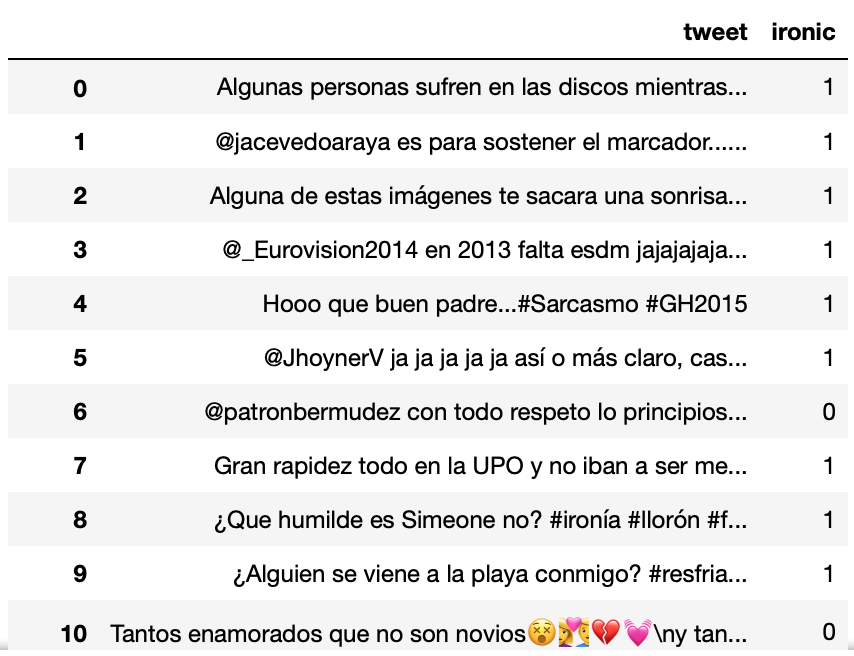
\includegraphics[width=\linewidth]{img/dataset.png}
	\caption{Dataset}
	\label{fig:dataset}
\end{figure}

\section{Preprocessing}
\label{sec:preprocessing}
The preprocessing stage is conceived to dispose of any information that will not be needed during the \ac{ml} step~\cite{preprocess}. The preprocessing was applied individually to each tweet.
The changes in the dataset that have been made are:
\begin{itemize}
	\item \textit{False items}: Since almost half the dataset tweets come from tweeter, it was required to download those tweets from the social network. Some of the captured tweets were false.
	\item \textit{Categorical values}: Originally the labels of the dataset were either 'True' or 'False'. These two values were encoded into 'True'= 1 and 'False' = 0.
	\item \textit{Stopwords}:  In \ac{ml} it is a very common practice to delete words which barely provide any information to the text (e.g. 'a', 'I', 'you'). In this project, the list of stopwords was chosen for the spanish language due to the language of the tweets. The list of words can be consulted in~\cite{stopwords}.
	\item \textit{Tokenization}:This process consists of splitting a string (tweet) into tokens. Usually a token is the same as a word.
	\item 
	\textit{Stemming}: This process consists of reducing the tokens into its root. Basically the words are transformed into its root. Stemming was accomplished using a Snowball stemmer. 
\end{itemize}
These steps of preprocessing were all executed defining a custom tokenizer but the categorical value encoding and the false item removal, which were done previously.\\
It is noteworthy to mention that the custom tokenizer is used later for the feature extraction.\\
At the beginning of the preprocessing stage, the dataset is split into two parts, a training part and a testing part. The purpose of this split is to train a clasifier using the train  sequence and evaluate the accuracy of the classifier using the test sequence. The split is taken randomly. The size of each sequence is 75\% for the train sequence and 25\% for the test sequence (8311 and 2771). More information on can be found on \cref{sec:modcons}.
\section{Feature Extraction}
\label{sec:feature}
 The feature extraction process consist of reading the text and extracting certain features. Furthermore, those extracted features will be fed to the classifier and finally the model will be completed. As a result, the accuracy of the model will be directly related to the choice of features. Therefore, it is very important to choose wisely the features to extract.\\
This section will be committed to extensively explaining the selected features.
\par
The extraction will be performed inside a Pipeline, which will execute each extraction sequentially. In this project, two pipelines are defined, the first aims at extracting the ngrams. With the ngrams extracted from the first pipeline, a second one will extract other features and unify the ngrams with the other extracted features. Even though there are two pipelines defined, the results of the ngrams pipeline are added to the other pipeline. This is done thanks to the Feature Union class provided by Scikit-Learn.
\subsection{Lexical Features}
Usually extracting lexical features involves getting the number of sentences and the number of words in each sentence. However, since this projects' dataset is made out of tweets and the number of characters in a tweet is limited, I have considered that each tweet contains only one sentence. As a consequence, the lexical feature extraction becomes very simple. The extraction consists of tokenizing each sentence and stemming each token (or word) to get the root. At the same time, the words belonging to the spanish stop list are removed (see \cref{sec:preprocessing} for more details). In~\cref{sec:tfidf} is explained what happens with the extracted words in this stage.
\subsection{Syntactic Features}
\todo[inline]{Esto no aparece en el código}
The syntactic feature extraction consists of counting the number of nouns, adjectives, verbs, adverbs, conjunctions, pronouns and numbers present in each tweet. In~\cref{sec:tfidf} is explained what happens with the extracted words in this stage.
\subsection{Ngram Features. Pipeline}
Ngram extractions consist of grouping the words into bag of words. If we group the words individually then a sentence with five words will be considered as a five words sentence. If we group two words together then a sentence of six words will be considered as a three word sentence. So each pair of words are understood by the estimator as one.\\
Since it is very difficult to guess what is the optimum bag of words (i.e. number of words) CountVectorizer method provided by the Scikit-Learn class allows us to define a range. Finally, to select the optimum range, a~\ac{gs} will be performed (see~\cref{sec:gs}).
\subsection{\acf{lda} Features}
\ac{lda}~\footnote{\url{https://en.wikipedia.org/wiki/Latent_Dirichlet_allocation}} is a generative statistical model that allows sets of observations to be explained by unobserved groups that explain why some parts of the data are similar.\\ In other words, \ac{lda} extraction can be used to extract how many topics are being spoken about in the dataset. This can be observed by analyzing each words' presence.\\
The main parameter of this statistical model is the number of topics. Similarly as with the ngrams features, a~\ac{gs} will be performed to find the optimum number of topics (see~\cref{sec:gs}).
\subsection{\acf{tfidf}}
\label{sec:tfidf}
\ac{tfidf}~\footnote{\url{https://en.wikipedia.org/wiki/Tf–idf}} is a numerical statistic that is intended to reflect how important a word is to a document in a collection or corpus. Particularly, the \ac{tfidf} recognizes those words that are rare in the corpus but may be of great importance. The \ac{tfidf} uses a word as an argument and outputs the inverse frequency of that word.\\
The equation used is~\cite{tfidf}:
\begin{equation}
\label{ec:tf}
	tf_{t,d} = \frac{count(t)}{count(alltermsindocument)}
\end{equation}
with
\begin{equation}
\label{ec:idf}
	idf_t=log(\frac{N}{df_t})
\end{equation}
and
\begin{equation}
\label{ec:tfidf}
	tfidf_{t,d}=tf_{t,d}\times idf_t
\end{equation}
The number of occurences of a word in a complete document is computed with~\cref{ec:tf}.~\Cref{ec:idf} represents the $idf$ of a word. That amount serves as how much information a word provides. As explained before, terms with less frequency are considered to provide more information to the whole document as more common terms. Finally,~\cref{ec:tfidf} computes the weight of a word.
\section{Classifiers}
\label{sec:clasif}
This section will explain extensively the classifiers used for the learning process.\\
Classification~\cite{classif} is the task of predicting the class to which an object, known as pattern, belongs. The pattern is assumed to belong to one and only one among a number of a priori known classes. Each pattern is uniquely represented by a set of measurements, known as features. One of the early stages in designing a classification system is to select an appropriate set of feature variables. These should “encode” as much class-discriminatory information, so that, by measuring their value for a given pattern, to be able to predict, with high enough probability, the class of the pattern. 
\begin{figure}
	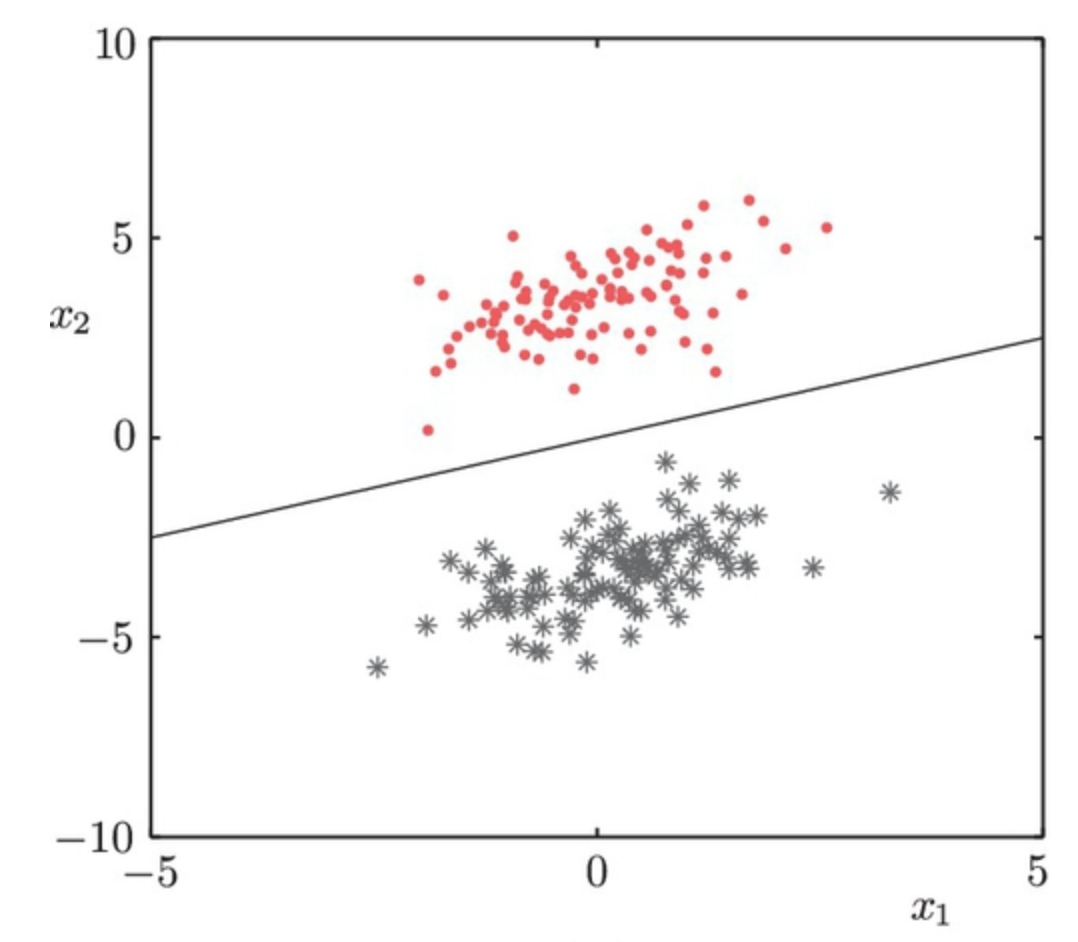
\includegraphics[width=\linewidth]{img/classifier.png}
	\caption{Classifier~\cite{classif}}
	\label{fig:classifier}
\end{figure}
\Cref{fig:classifier} is an example of two linearly separable classes, where a straight line can separate the two classes. \\
In this project, there will be three classifiers.
\subsection{\acf{nb}}
The~\ac{nb} classifier is a typical and popular example of a suboptimal classifier. The basic assumption is that the components (features) in the feature vector are statistically independent; hence, the joint~\ac{pdf} can be written as a product of $l$ marginals~\cite{classif}:
\begin{equation}
	p(x|\omega_i)=\prod_{k=1}^{l}p(x_k|\omega_i)
	\label{ec:nb}
\end{equation}
Considering that both $\omega_i$ and $x$ are Gaussian variables, it is only necessary to compute the mean and the variance for each pair of variables. That leads to a total of $2\times l$ unknown variables for a subclass. Computationally speaking, $2\times l$ complexity is achievable in a reasonable amount of time for a large $l$. This is the great advantage of the \ac{nb}.\par
The \ac{nb} classifier was defined setting the parameter $alpha = 0.01$. Nevertheless, it is not very important what parameters to set when defining the classifier since a \ac{gs} will be performed with the purpose of discovering the best classifier parameters. (See~\cref{sec:gs})
In this project, the results obtained for the~\ac{nb} with no parameter optimization can be observed in~\cref{tab:nb1}.
\begin{table}[h!]
	\centering
	\begin{tabular}{||c c c c c||} 
		\hline
		Variable & Precision & Recall & F1-Score & Support \\ [0.5ex] 
		\hline\hline
		0 & 0.81733 & 0.78781 & 0.80230 & 1329 \\ 
		1 & 0.81074 & 0.83773 & 0.82401 & 1442 \\
		avg/total & 0.81390 & 0.81379 & 0.81360 & 2771 \\
		[1ex] 
		\hline
	\end{tabular}
		\caption{\acl{nb} Classification Report}
		\label{tab:nb1}
\end{table}
The quality of a classifier will be established using the \textit{F1-Score} field from the classification report. For more details about this precedent see~\cref{sec:score}.
\subsection{\acf{svm}}
Support vector machine~\cite{svm} is a supervised learning algorithm that can be used for classification and regression. It is able to classify data linearly and nonlinearly using kernel methods. Each data point in the training dataset is labeled, as it is supervised learning, and mapped to the input feature space, and the aim is to classify every point of new data to one of the classes. A data point is an N dimension number, as N is the number of features, and the problem is to separate this data using N-1 dimensional hyperplane and this is considered to be a linear classifier.\par
The~\ac{svm} was defined setting as parameters \textit{C} = 1 and \textit{kernel} = linear. In other words, the initial~\ac{svm} model was the linear~\ac{svm} model.\\
With such parameters, the results can be observed in~\cref{tab:sv1}. The quality of the classifier was established following the \textit{F1-Score} field from the classification report. For more details see~\cref{sec:score}. 

\begin{table}[h!]
	\centering
	\begin{tabular}{||c c c c c||} 
		\hline
		Variable & Precision & Recall & F1-Score & Support \\ [0.5ex] 
		\hline\hline
		0 & 0.92590 & 0.92387 & 0.92488 & 1366 \\ 
		1 & 0.92614 & 0.92811 & 0.92712 & 1405 \\
		avg/total & 0.92602 & 0.92602 & 0.92602 & 2771 \\
		[1ex] 
		\hline
	\end{tabular}
	\caption{\acl{svm} Classification Report}
	\label{tab:sv1}
\end{table}
\subsection{\acf{knn}}
\ac{knn} is based on the idea that samples that are close with respect to a predefined distance metric are also similar, so they can share their peculiar features. To measure that distance, a distance function is defined. Usually, that distance function is the Minkowski metric~\cite{countvect1}. For each data point in the out-sample data, we calculate its distance from all data points in the in-sample data. Each data point has a vector of distances and the K distance which is close enough will be selected and the final decision about the class of the data point is based on a weighted combination of all k neighborhoods~\cite{svm}.\par
The~\ac{knn} was defined setting as parameters \textit{neighbors} = 7.\\
The results can be observed in~\cref{tab:knn1}. The quality of the classifier was established following the \textit{F1-Score} field from the classification report. For more details see~\cref{sec:score}. 
\begin{table}[h!]
	\centering
	\begin{tabular}{||c c c c c||} 
		\hline
		Variable & Precision & Recall & F1-Score & Support \\ [0.5ex] 
		\hline\hline
		0 & 0.79561 & 0.76940 & 0.78229 & 1366 \\ 
		1 & 0.78276 & 0.80783 & 0.79510 & 1405 \\
		avg/total & 0.78909 & 0.78888 & 0.78878 & 2771 \\
		[1ex] 
		\hline
	\end{tabular}
	\caption{\acl{knn} Classification Report}
	\label{tab:knn1}
\end{table}
\subsection{\acf{lr}}
 \acl{lr} is a classification method that is based on the probability of a sample belonging to a class.
 It consists of maximum-entropy classification. Mathematically, the aim is to compute the minimum of~\cref{ec:lr}~\cite{lr}.
 \begin{equation}
 	min_{w,c}\frac{1}{2}w^{T}w+C\sum_{i=1}^{n}log(exp(-y_i(X_i^{T}w+c))+1)
 	\label{ec:lr}
 \end{equation}
 The~\ac{lr} classifier was defined setting the parameter \textit{C} = 1. \\
 For such a parameter, the results obtained can be observed in~\cref{tab:lr1}. The quality of the classifier was established following the \textit{F1-Score} field from the classification report. For more details see~\cref{sec:score}.
 
 \begin{table}[h!]
 	\centering
 	\begin{tabular}{||c c c c c||} 
 		\hline
 		Variable & Precision & Recall & F1-Score & Support \\ [0.5ex] 
 		\hline\hline
 		0 & 0.90007 & 0.90074 & 0.90040 & 1360 \\ 
 		1 & 0.90426 & 0.90361 & 0.90393 & 1411 \\
 		avg/total & 0.90220 & 0.90220 & 0.90220 & 2771 \\
 		[1ex] 
 		\hline
 	\end{tabular}
 	\caption{\acl{lr} Classification Report}
 	\label{tab:lr1}
 \end{table}
 
\section{Quality of a Classfier}
\label{sec:score}
In order to ensure a sufficient classifier accuracy, precision is not always the best indicator. Let us consider a binary class dataset where 99\% of the data belongs to one class and only 1\% of the data belongs to the other class. Now, if a classifier were to always predict the majority class for every data point, it would have 99\% accuracy. But that would not mean that the classifier is performing well. To have a better idea of the classifiers' efficiency we first must define some parameters~\cite{f1score}:
\begin{itemize}
	\item \textit{\acf{tp}}: Cases where the actual and the predicted classes are both positive.
	\item \textit{\acf{tn}}: Cases where the actual and the predicted classes are both negative.
	\item \textit{\acf{fp}}: Cases where the actual class is negative but the predicted class is positive.
	\item \textit{\acf{fn}}: Cases where the actual class is positive but the predicted class is negative.
\end{itemize}
To better understand these definitions let us imagine a classifier that predicts a sarcastic when in fact that tweet is not sarcastic, that would be a false positive. On the other hand, if the classifier predicts that a tweet is not sarcastic when in reality is sarcastic, that would be a false negative.
\subsection{Precision}
Precision is defined as the ratio of number of positive cases that were correct to all the cases that were identified as positive~\cite{f1score}. Mathematically:
\begin{equation}
	Precision = \frac{\ac{tp}}{\ac{tp}+\ac{fp}}
	\label{ec:precision}
\end{equation}
\subsection{Recall}
Recall is defined as the ratio of the number of positive cases that were identified to the all positive cases present in the dataset~\cite{f1score}. Mathematically:
\begin{equation}
	Recall = \frac{\ac{tp}}{\ac{tp}+\ac{fn}}
	\label{ec:recall}
\end{equation}
\subsection{F1 Score}
is the harmonic average of the precision and recall. It is a metric that conveys the balance between precision and recall~\cite{f1score}. Mathematically:
\begin{equation}
	F1 = 2\times \frac{Precision \times Recall}{Precision + Recall}
	\label{ec:f1score}
\end{equation}
Since the F1 score takes into account both the precision and the recall (see~\cref{ec:f1score}), it is the most suitable for determining a binary classifiers' quality. In this project, a tweet can either be sarcastic or non-sarcastic. Therefore, F1 score report is the appropiate quality measure.
\subsection{Model Creation}
\label{sec:modcons}
The~\cref{fig:modcons} depicts the methodology followed for training and evaluating the classifier. Firstly, the dataset is split into two sets, the training and the test. (In the~\cref{fig:modcons}, there is another subdivision called \textit{val} but that will not be necessary in this project). Once the split is done, a model is constructed. Finally, the quality of that model is evaluated using the test set and applying the F1 score.
\begin{figure}
	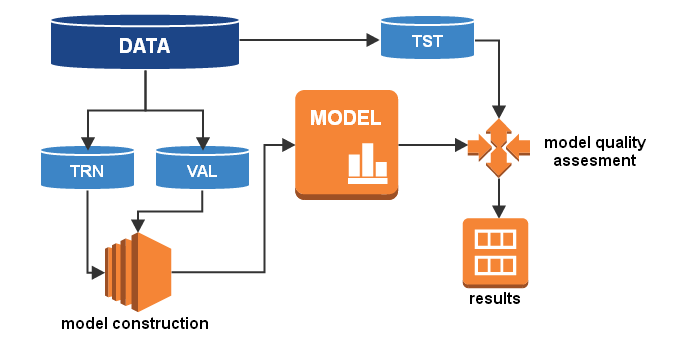
\includegraphics[width=\linewidth]{img/model_construction.png}
	\caption{Model Construction~\cite{modcons}}
	\label{fig:modcons}
\end{figure}
\section{Parameter Optimization}
This section will cover how was the parameter optimization performed and what were the results obtained for each classifier.\\
To understand the parameter optimization, first we must comprehend how is the classifier built in this project.\\
The simplest definition of text classification is that it is a classification of text based on the content of that text. Now, in general, all the machine learning methods and algorithms are written for numeric features/variables. One of the most important problems with text corpus is how to represent text as numeric features~\cite{lr}. That stage is accomplished by making use of the pipeline described in~\cref{sec:feature}. Depending on how the feature extraction pipeline was created, the parameters of the final classifier change. Therefore, the classifier is assembled by both the pipeline described in~\cref{sec:feature} and one of the classifiers chosen in~\cref{sec:clasif}.\\
In order to find the right classifier parameters, it must be carried out a parameter search for the pipeline parameters and the classifier parameters.\\
From~\cref{sec:feature}, the pipeline extracts three main features; ngrams, words (custom tokenizer) and topics (\ac{lda}). From these features, the only parameters that will be searched are the number of topics from~\ac{lda} and the number of ngrams.\\
From~\cref{sec:clasif}, the parameters searched will depend on the type of classifier. On the following subsections from this section, the topics will be covered.
The parameter search will be done using the GridSearchCV from the Scikit Learn class. The principle of the GridSearchCV is:
\begin{enumerate}
	\item Define a dictionary of parameters to change.
	\item Fit the grid search with the train dataset (this process can take a very long time).
	\item Print best score alongside with the best parameters.
	\item Print the metrics accuracy score by testing the classifier with the best parameters found. For this, it is required a test dataset.
\end{enumerate}
\subsection{Grid Search}
\label{sec:gs}
A grid search is an exhaustive search through a manually-specified subset of the hyperparameter space. The grid search algorithm requires a performance metric, such as cross-validation error or validation-set error to evaluate the best possible parameter~\cite{gs}. The grid search method comes from the Scikit Learn class.\\
A grid search was optimizied for each classifier to get the best performance. 
\subsubsection{\acl{nb}}
\begin{itemize}
	\item \textbf{Parameters to optimize}:
	\begin{enumerate}
		\item \textit{Alpha}. Belongs to classfier
		\item \textit{Number of topics}. Belongs to pipeline
	\end{enumerate}
	\item \textbf{Results}
		\begin{table}[h!]
			\centering
			\begin{tabular}{||c c c c c||} 
				\hline
				Variable & Precision & Recall & F1-Score & Support \\ [0.5ex] 
				\hline\hline
				0 & 0.96481 & 0.96765 & 0.96623 & 1360 \\ 
				1 & 0.96873 & 0.96598 & 0.96735 & 1411 \\
				avg/total & 0.96680 & 0.96680 & 0.92602 & 2771 \\
				[1ex] 
				\hline
			\end{tabular}
			\caption{\acl{nb} Classification Report Optimized}
			\label{tab:nb2}
		\end{table}
	
\end{itemize}

\subsubsection{\acl{svm}}
\begin{itemize}
	\item \textbf{Parameters to optimize}:
	\begin{enumerate}
		\item \textit{C}. Belongs to classfier
		\item \textit{Number of topics}. Belongs to pipeline
		\item \textit{NUmber of ngrams}. Belongs to pipeline
		
	\end{enumerate}
	\item \textbf{Results}
	\begin{table}[h!]
		\centering
		\begin{tabular}{||c c c c c||} 
			\hline
			Variable & Precision & Recall & F1-Score & Support \\ [0.5ex] 
			\hline\hline
			0 & 0.91131 & 0.90662 & 0.90896 & 1360 \\ 
			1 & 0.91044 & 0.91495 & 0.91269 & 1411 \\
			avg/total & 0.91086 & 0.91086 & 0.91086 & 2771 \\
			[1ex] 
			\hline
		\end{tabular}
		\caption{\acl{svm} Classification Report Optimized}
		\label{tab:sv2}
	\end{table}
	
\end{itemize}
\subsubsection{\acl{knn}}
Since the results of the~\ac{knn} were very low (see~\cref{tab:knn1}) there was no grid search performed to predict the best classifier parameters. Furthermore,~\ac{knn} it is not a recommended classifier for the porpose of the project.
\subsubsection{\acl{lr}}
\begin{itemize}
	\item \textbf{Parameters to optimize}:
	\begin{enumerate}
		\item \textit{Number of topics}. Belongs to pipeline
	\end{enumerate}
	\item \textbf{Results}
	\begin{table}[h!]
		\centering
		\begin{tabular}{||c c c c c||} 
			\hline
			Variable & Precision & Recall & F1-Score & Support \\ [0.5ex] 
			\hline\hline
			0 & 0.90007 & 0.90074 & 0.90040 & 1360 \\ 
			1 & 0.90426 & 0.90361 & 0.90393 & 1411 \\
			avg/total & 0.90220 & 0.90220 & 0.90220 & 2771 \\
			[1ex] 
			\hline
		\end{tabular}
		\caption{\acl{lr} Classification Report Optimized}
		\label{tab:lr2}
	\end{table}
	
\end{itemize}




